\documentclass[border=2pt]{standalone}

\usepackage{tikz}
\usetikzlibrary{petri}

\begin{document}

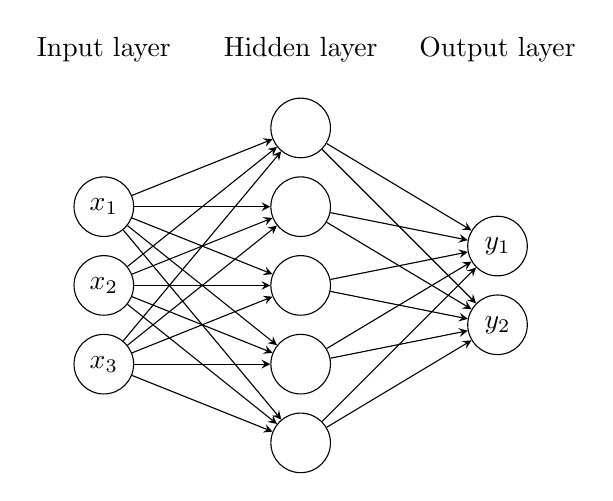
\begin{tikzpicture}
    \newcommand{\inputnum}{3}
    \newcommand{\hiddennum}{5}
    \newcommand{\outputnum}{2}
    \node[] at (0, 1) {Input layer};
    \node[] at (2.5, 1) {Hidden layer};
    \node[] at (5, 1) {Output layer};
    % Input layer
    \foreach \i in {1, ..., \inputnum} {
            \node[place] (Input-\i) at (0, -\i) {$ x_\i $};
        }
    % Hidden layer
    \foreach \i in {1, ..., \hiddennum} {
            \node[place, yshift=(\hiddennum-\inputnum)*1cm/2] (Hidden-\i) at (2.5, -\i) {};
        }
    % Output layer
    \foreach \i in {1, ..., \outputnum} {
            \node[place, yshift=(\outputnum-\inputnum)*1cm/2] (Output-\i) at (5, -\i) {$ y_\i $};
        }

    % Connect layers
    \foreach \i in {1, ..., \inputnum} {
            \foreach \j in {1, ..., \hiddennum} {
                    \draw[-stealth] (Input-\i) -- (Hidden-\j);
                }
        }
    \foreach \i in {1, ..., \hiddennum} {
            \foreach \j in {1, ..., \outputnum} {
                    \draw[-stealth] (Hidden-\i) -- (Output-\j);
                }
        }
\end{tikzpicture}

\end{document}